% Author: Andrei Tumbar

\documentclass[11pt]{article}
    \title{\textbf{Homework 9}}
    \author{Andrei Tumbar}
    \date{03-31-2021}

\usepackage{pgf}
\usepackage{tikz}
\usetikzlibrary{arrows,automata}
\addtolength{\topmargin}{-1.2in}
\begin{document}
\maketitle

\section*{Exercise 24}

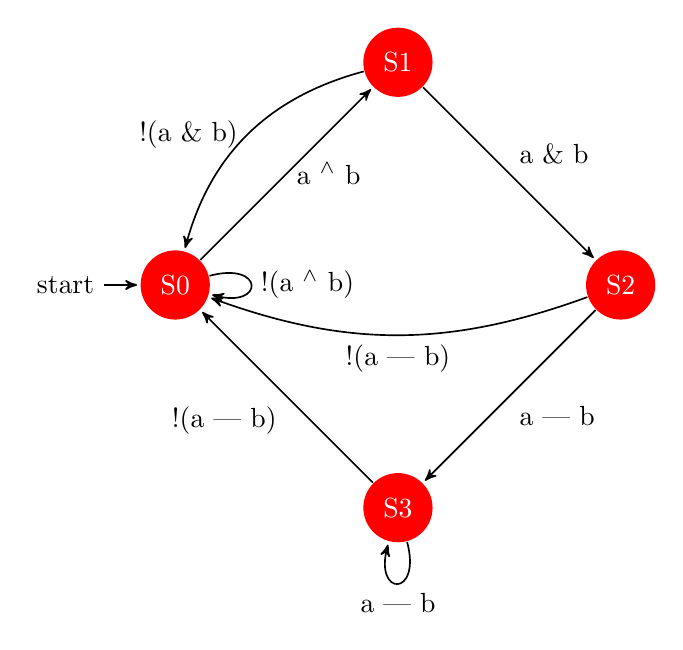
\begin{tikzpicture}[->,>=stealth',shorten >=1pt,auto,node distance=4cm,
                    semithick]
	\tikzstyle{every state}=[fill=red,draw=none,text=white]

	\node[initial,state] (A)                    {S0};
	\node[state]         (B) [above right of=A] {S1};
	\node[state]         (D) [below right of=A] {S3};
	\node[state]         (C) [below right of=B] {S2};

	\path (A)	edge [right]		node{a \textsuperscript{$\wedge$} b} (B)
				edge [loop right] 	node{!(a \textsuperscript{$\wedge$} b)} (A)
		
		  (B)	edge				node{a \& b} (C)
		  (B)	edge [bend right=30, left]	node{!(a \& b)} (A)
		  
		  (C)	edge				node{a | b} (D)
		  (C)	edge [bend left=20] node {!(a | b)} (A)
		
		  (D)	edge [loop below]	node{a | b} (D)
		  (D)	edge				node{!(a | b)} (A)
		;
\end{tikzpicture}

\end{document}
